\documentclass[a4paper,12pt]{article} % тип документа

% Поля страниц
\usepackage[left=2.5cm,right=2.5cm,top=1.5cm,bottom=2cm,bindingoffset=0cm]{geometry}
    
% Отступ после заголовка
\usepackage{indentfirst}

% Картинки
\usepackage{graphicx}
\graphicspath{{images/}}
\usepackage{placeins}

% Таблицы
\usepackage{booktabs}
% \usepackage{floatrow}
\usepackage{subcaption}

% Русский язык
\usepackage{cmap}  % поиск в PDF
\usepackage{mathtext}  % русские буквы в формулах
\usepackage[T2A]{fontenc}  % кодировка
\usepackage[utf8]{inputenc}  % кодировка исходного текста
\usepackage[english,russian]{babel}  % локализация и переносы

% Математика
\usepackage{amsmath}

% Ссылки TODO
% \usepackage[unicode=true]{hyperref}
% \usepackage[T1]{fontenc}

\begin{document}

\begin{center}   
	\large{Работа 2.3.1\\\textbf{Получение и измерение вакуума}}\\
\end{center}

\section{Аннотация}

\noindent\textbf{Цель работы:}
1) измеренеи объёмов форвакуумной и высоковакуумной частей установки; 2) определение скорости откачки системы в стационарном режиме, а также по ухудшению и по улучшению вакуума.
	
\smallskip
\noindent\textbf{В работе используются:}
вакуумная установка с манометрами: масляным, термопарным и ионизационным.

\section{Теоретические сведения}

\subsection*{Процесс откачки}

Производительность насоса определяется скоростью откачки $W$ (л/с): $W$ — это объем газа, удаляемого из сосуда при данном давлении за единицу времени. Скорость откачки форвакуумного насоса равна емкости воздухозаборной камеры, умноженной на число оборотов в секунду.
Рассмотрим обычную схему откачки. Разделим вакуумную систему на две части: «откачиваемый объем» (в состав которого включим используемые для работы части установки) и «насос», к которому, кроме самого насоса, отнесем трубопроводы и краны, через которые
производится откачка нашего объема. Обозначим через $Q_d$ количество газа, десорбирующегося с поверхности откачиваемого объема в единицу времени, через $Q_i$ — количество газа, проникающего в единицу времени в этот объем извне — через течи. Будем считать, что насос обладает скоростью откачки $W$ и в то же время сам является источником газа; пусть $Q_n$ — поток газа, поступающего из насоса назад в откачиваемую систему. Будем измерять количество газа $Q_d$, $Q_i$ и $Q_n$ в единицах $PV$ (легко видеть, что это произведение с точностью до множителя $RT/ \mu$ равно массе газа). Основное уравнение, описывающее процесс откачки, имеет вид

\begin{equation}
\label{otkachka}
	-VdP=(PW-Q_d-Q_n-Q_i)dt.
\end{equation}

Левая часть этого уравнения равна убыли газа в откачиваемом объеме $V$ , а правая определяет количество газа, уносимого насосом, и количество прибывающего вследствие перечисленных выше причин
за время $dt$. При достижении предельного вакуума (давление $P_{pr}$)

\begin{equation}
\label{predel_1}
	\frac{dP}{dt}=0,
\end{equation}

\begin{equation}
\label{predel_2}
	W=\frac{\sum Q_i}{P_{pr}}.
\end{equation}

Обычно $Q_i$ постоянно, a $Q_n$ и $Q_d$ слабо зависят от времени, поэтому в наших условиях все эти члены можно считать постоянными. Считая также постоянной скорость откачки $W$ , уравнение~(\ref{otkachka}) можно проинтегрировать и, используя~(\ref{predel_1}), получить
\begin{equation}
\label{davlenie}
	P = P_o \exp{(-\frac{W}{V} t)} + P_{pr}.
\end{equation}

\subsection*{Течение газа через трубу}

Характер течения газа существенно зависит от соотношения между размерами системы и длиной свободного пробега молекул. При атмосферном давлении и даже при понижении давления до форвакуумного длина свободного пробега меньше диаметра трубок и течение откачиваемого газа определяется его вязкостью, т. е. взаимодействием его молекул. При переходе к высокому вакууму картина меняется. Столкновения молекул между собой начинают играть меньшую роль, чем соударения со стенками. Течение газа в трубе напоминает в этих условиях диффузию газа из области больших концентраций в области, где концентрация ниже, причем роль длины свободного пробега играет ширина трубы.
Для количества газa, протекающего через трубу в условиях высокого вакуума или, как говорят, в кнудсеновском режиме, справедлива формула

\begin{equation}
\label{formula}
	\frac{d(PV)}{dt}=\frac{4}{3}r^3 \sqrt{\frac{2\pi RT}{\mu}} \frac{P_2-P_1}{L}.
\end{equation}

Применим эту формулу к случаю, когда труба соединяет установку с насосом.
Пренебрежем давлением $P_1$ у конца, обращенного к насосу. Будем измерять количество газа, покидающего установку при давлении $P = P_2$. Пропускная способность трубы

\begin{equation}
	C_{tr}=(\frac{dV}{dt})_{tr}=\frac{4}{3}\frac{r^3}{L}\sqrt{\frac{2\pi RT}{\mu}}.
\end{equation}

Мы видим, что пропускная способность зависит от радиуса трубы в третьей степени и обратно пропорциональна ее длине. В вакуумных установках следует поэтому применять широкие короткие  трубы.

При расчете вакуумных систем нужно принимать во внимание также пропускную способность отверстий, например, в кранах. Для диффузионного насоса можно считать, что каждая молекула воздуха, попавшая в кольцевой зазор между соплом и стенками насоса, увлекается струей пара и не возвращается обратно в откачиваемый объем. Скорость откачки такого насоса можно считать равной пропускной способности отверстия с площадью, равной площади кольцевого зазора, т. е. насос качает как кольцевой зазор, с одной стороны которого расположен откачиваемый объем, а с другой -- пустота.

\newpage

\section{Используемое оборудование}

\begin{figure}[h!]
    \centering
    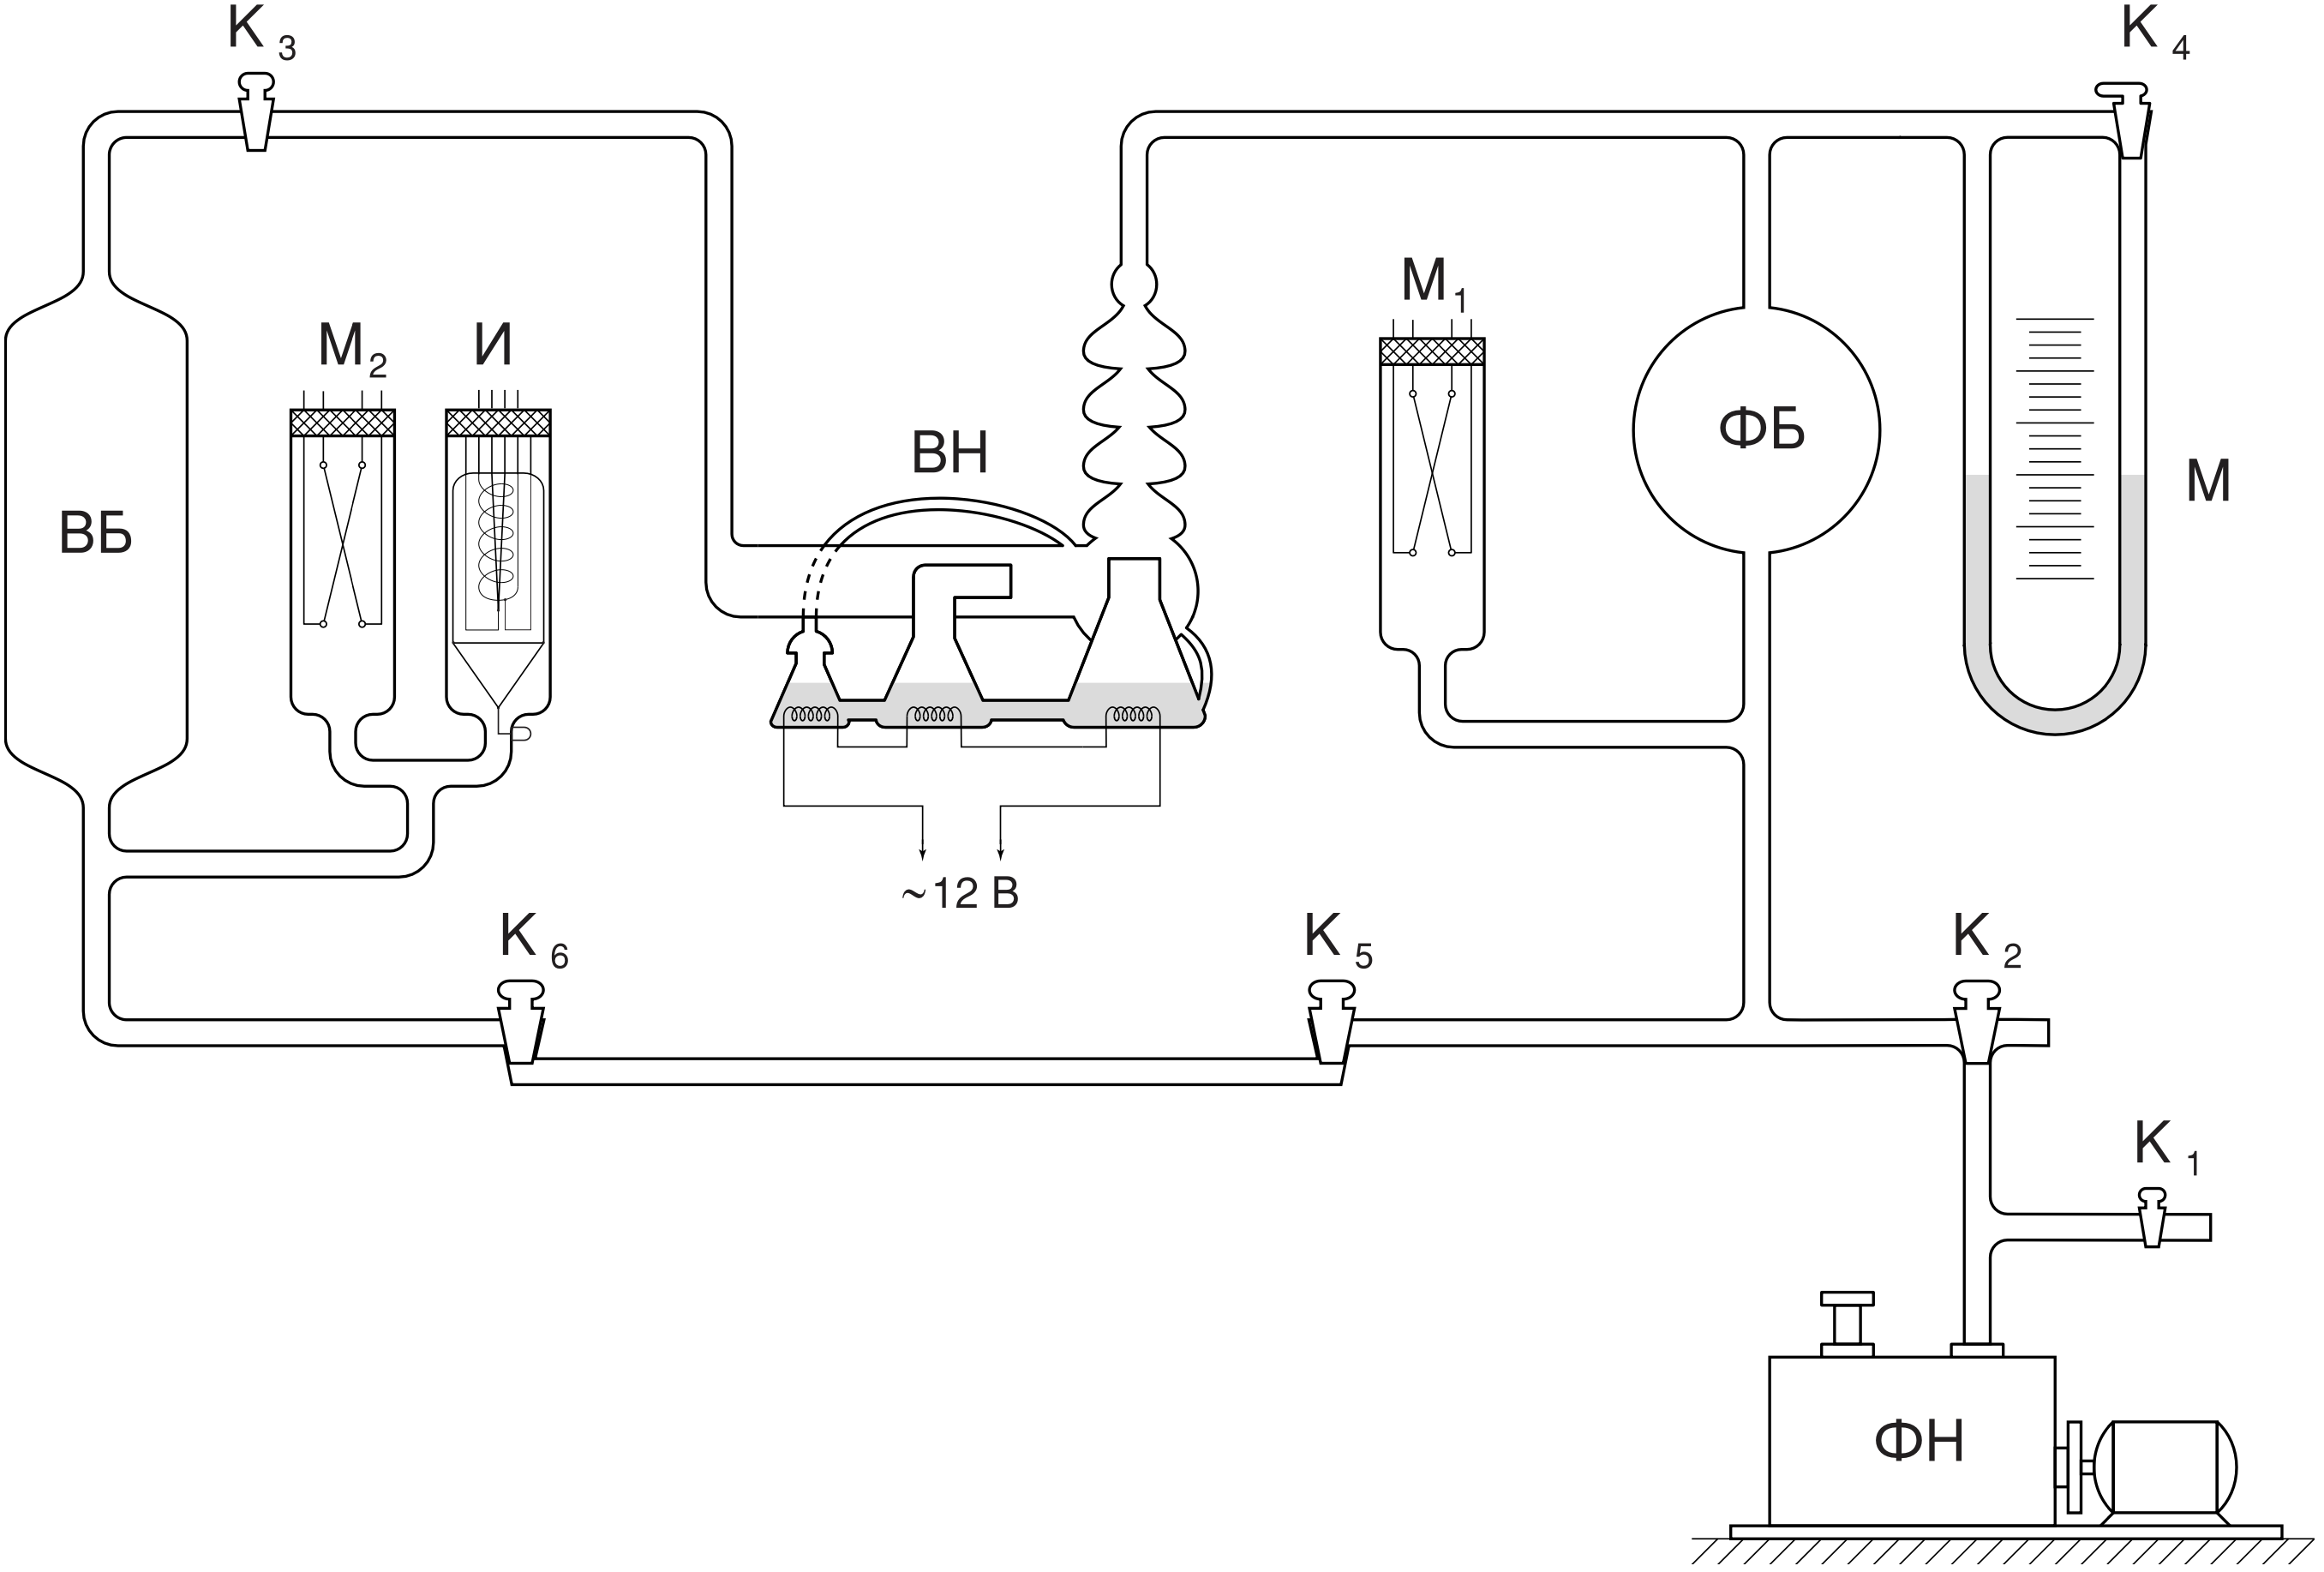
\includegraphics[width=\textwidth]{установка.png}
    \caption{Схема экспериментальной установки}\label{setup}
\end{figure}

\FloatBarrier

\section{Методика измерений}

\begin{enumerate}

	\item
		Определим объемы форвакуумной и высоковакуумной частей установки. Сначала впустим атмосферу в установку. Запрем воздух при комнатных условиях в капилляре между кранами 5 и 6. После этого откачаем воздух из оставшейся части установки (сделав это в два этапа - сначала насос должен откачать сам себя, а только потом - установку). После этого мы сначала высвободим запертый воздух только в ФВ часть, а затем добавим к ней и ВВ. Тогда записав уравнение Менделеева-Клапейрона и зная объем капилляра, мы найдем объемы соответствующих частей установки:
	\begin{equation}
		P_0 V_0 = P_v (V_f + V_v),
	\end{equation}
	где $P_0$ -- атмосферное давление; $V_0$ -- объем капилляра и кранов 5 и 6; $P_v$ -- установившееся давление; $V_f$ и $V_v$ -- соотвественно объемы форвауумной и высоковакуумной частей.
		
	\item
		Для измерения скорости откачки диффузионного насоса измерим улучшение вакуума во времени. Построим график зависимости $-\ln{\frac{P-P_{pr}}{P_0}}$ от $t$. Из формулы~(\ref{davlenie}) следует, что наклон, построенной кривой, есть $W / V$
	
	\item
		Откроем кран 6 и создадим исскуственную течь через капилляр. Рассчитаем производительность насоса по различию $P_{pr}$ и $P_u$, где $P_u$ -- установившееся давление в высоковакуумной части с искусственной течью. В условиях высокого вакуума справдлива формула~(\ref{formula}), где положим $P_1 := P_u$, $P_2$ -- давление в форвакуумной части. 
	
\end{enumerate}

% \section{Результаты измерений и обработка данных}

% \section{Обсуждение результатов}

\end{document}
